\begin{frame}
\frametitle{Method for $N$ judges, $M$ objects and $K$ characteristics}
\begin{block}{Components}
\begin{itemize}
\item Ratings tensor : $X \in \mathbb{R}^{N\times M \times K}$
\item Reputation tensor : $R \in \mathbb{R}^{M\times K}$
\item Weight vector : $w \in \mathbb{R}^{N\times 1}$
\end{itemize}
\end{block}
\begin{block}{Two stages of the method}
\begin{itemize}
\item Preprocessing : possibly center the votes to zero and set variances to 1.
\item Iteration : determine weights of the judges and the final reputation
\end{itemize}
\end{block}
\end{frame}

\begin{frame}
\begin{block}{Two steps iteration}
\begin{itemize}
\item Reputation computation : weighted sum of the votes
$$R_{jk}^{t+1}(w,X) = \frac{\sum_{i}X_{ijk}w^t_{i}}{\sum_i w_{i}}$$
\item Filtering : The farther a judge $i$ rates from the reputation, the lesser its weight\\
Define the column vector $d^{ij} \in \mathbb{R}^K$ as follows :
$$ d^{ij}_k = X_{ijk}-R^{t+1}_{jk}$$
$$div_i =  \frac{1}{MK}\sum_{j} (d^{ij})^T (d^{ij})$$
$$w_i^{t+1}(X,r) = 1 -k \cdot div_i$$
with $k$ a constant 
\end{itemize}
\end{block}
\end{frame}
\begin{frame}
\frametitle{Example for one judge and one object for $K=2$}
\begin{block}{}
Weight according to $d^{ij}\in \mathbb{R}^{2\times 1}$
\begin{figure}
\centering
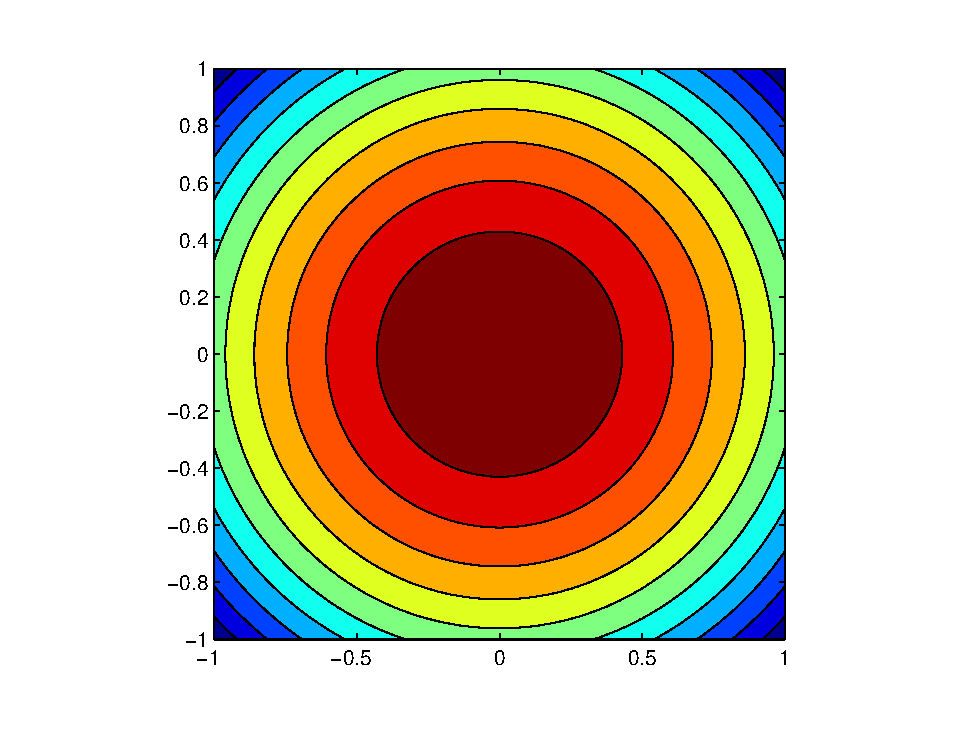
\includegraphics[width = 7cm]{../rapport/images/courbes.eps}
\end{figure}
We simply take the sum of this over all the objects
\end{block}
\end{frame}

\begin{frame}
\frametitle{Properties of the method}
\begin{block}{Energy function}
\begin{itemize}
\item Fix points of the iteration are stationary points of the energy function
$$E(r) =  \sum_{i=1}^n \int_0^{div_i(r)}g(u) du + c $$
\item The stationary point in the domain concerned is unique and is a strict minimum
\item The iteration corresponds to a steepest descent method step
\end{itemize}
\end{block}
\end{frame}